
\begin{figure}
    \centering
    
    \begin{subfigure}[t]{0.45\textwidth}
        \centering
        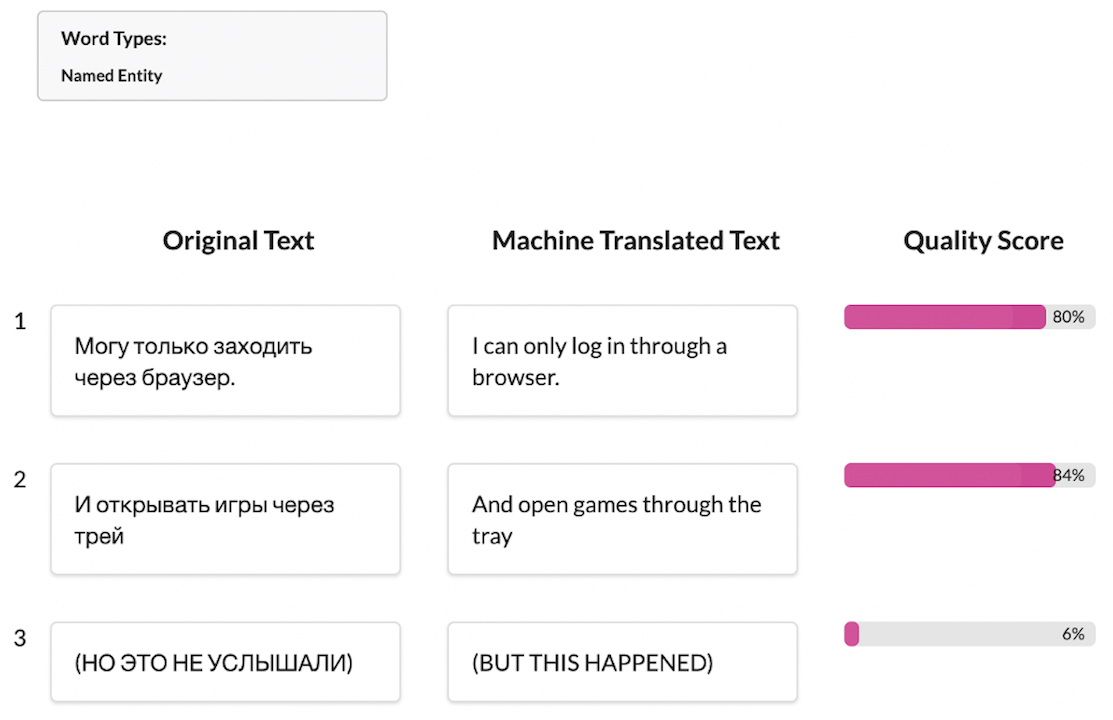
\includegraphics[width=\linewidth]{p1_v_0.png} 
        \caption{Passage 1 (passage type 1), Human Quality condition} \label{fig:p1_human_quality}
    \end{subfigure}
    \hfill
     \begin{subfigure}[t]{0.45\textwidth}
        \centering
        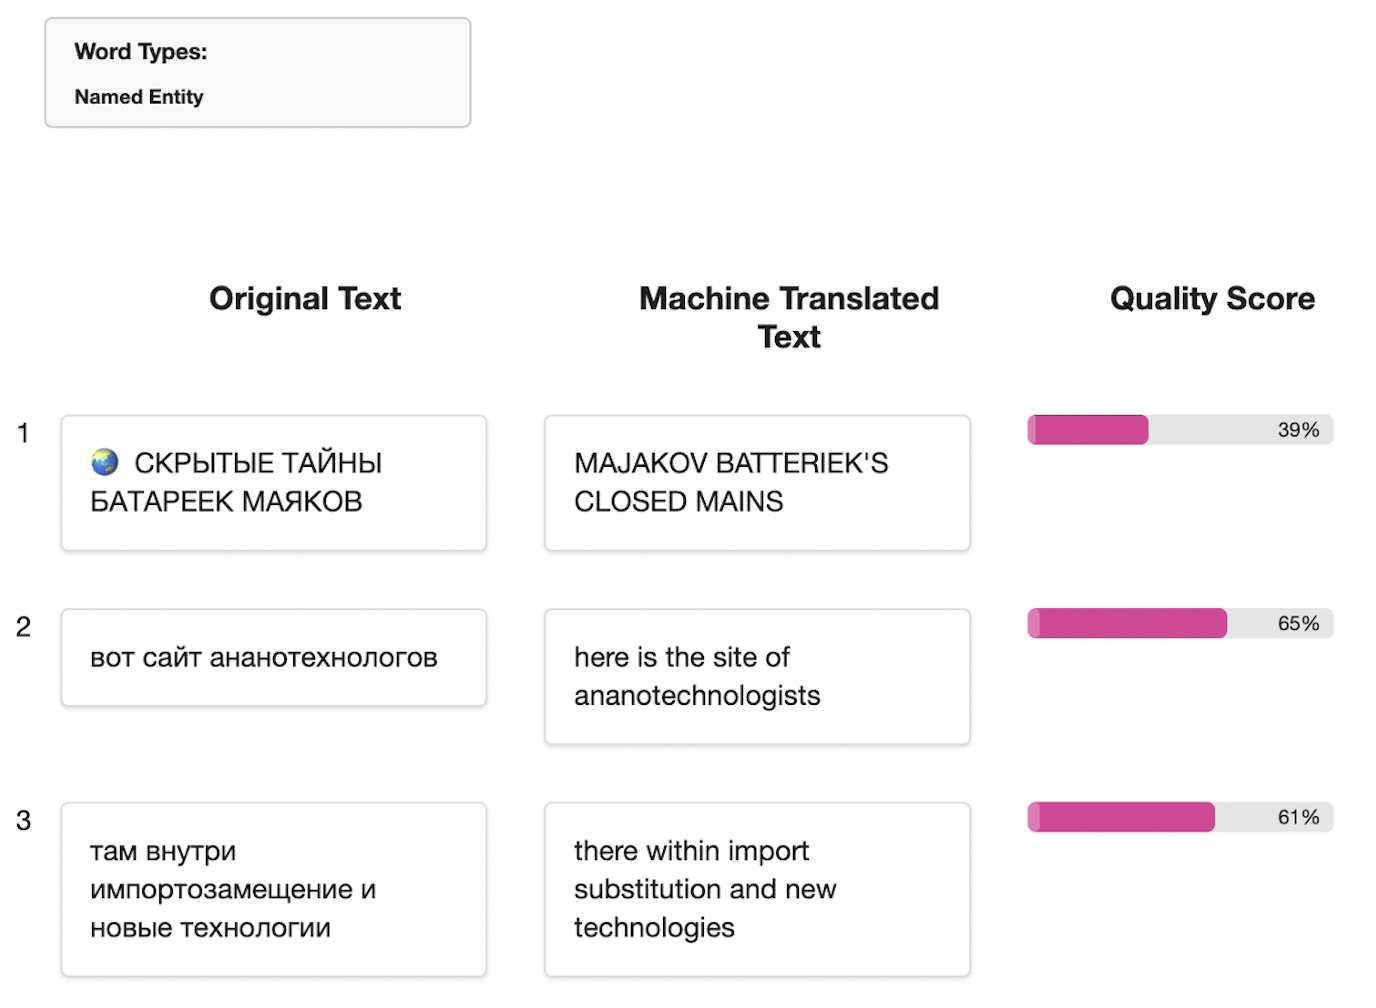
\includegraphics[width=\linewidth]{p3_p_0.png} 
        \caption{Passage 3 (passage type 2), Predicted Quality condition} \label{fig:p3_predicted_quality}
    \end{subfigure}
    
    \caption{Select examples of stimuli. All stimuli are available in supplemental materials.}
    \label{fig:exp_stim}
    
\end{figure}

\section{VeriCAT System Overview}
VeriCAT is designed to help analysts quickly and efficiently identify Russian $\rightarrow$ English MT sentences with poor translation quality, particularly in cases where fluency is a poor proxy for translation quality. %VeriCAT predicts quality scores for Russian $\rightarrow$ English translations generated by the pretrained FairSeq model~\cite{ott-etal-2019-fairseq} that performed best at WMT 2019 (news task, the most recent results from the annual benchmark for MT).
%VeriCAT is novel in that it uses QE as a means of communicating to the user whether a specific sentence of translated text is trustworthy. 
Commonly used MT accuracy metrics such as BLEU score~\cite{papineni-etal-2002-bleu} provide information about the accuracy of a MT model in general, (for example, FairSeq has a BLEU score of 40.0 on Russian to English translation, calculated with the SacreBLEU standard \cite{post-2018-call}) but, unlike VeriCAT, they do not provide feedback on individual translated sentences.  
%Our goal was to design a system that provides contextual information for \textit{individual snippets} of translated text, as opposed to the quality of the MT model as a whole.    
Below, we describe the training dataset for VeriCAT's QE model, the QE model itself, and VeriCAT's user interface.    

\subsection{Training Dataset}
The VeriCAT QE model is finetuned on a dataset composed of 7,000 labeled sentence pairs. The source of this text is passages from Reddit or Russian Proverbs from wikiquotes. The training dataset is curated from these sources because they represent types of text on which machine translation models are challenged. Each sentence is translated using the pretrained FairSeq model~\cite{ott-etal-2019-fairseq} that performed best at WMT 2019 (news task, the most recent results from the annual benchmark for MT). Each sentence has 3 Direct Assessment (DA) score quality judgments by human translators. These DA scores were labeled by ModelFront. Each DA score is rated on a scale from 1-100, with 100 representing a perfect translation. Across the dataset the average score is 68. These labeled data were also contributed to the World Machine Translation Workshop (Nov 2020) as part of the Quality Estimation Shared Task\footnote{statmt.org/wmt20}.  


\subsection{Quality Estimation Model}
Quality Estimation benchmarks are set annually at the World Machine Translation (WMT) QE Shared task. At the time of this study, the most accurate QE model available in the open source is the Predictor-Estimator model~\cite{Kim2017PredictorEstimatorUM}, open-sourced by OpenKiwi\footnote{https://github.com/Unbabel/OpenKiwi/tree/master/kiwi}~\cite{UnBabel} and the benchmark for WMT 2020. We pretrained the predictor model on the same parallel datasets the FairSeq translation model~\cite{ott-etal-2019-fairseq} was trained on. We finetuned the estimator model on the novel Russian-English QE dataset detailed above, tuning the following hyperparameters from the baseline model: epochs, hidden LSTM layers, learning rate, batch size, and dropout. We obtained a Pearson correlation of 0.62 on the development set, which we used to test since the shared task test set was not known to us. We ran inference with this model to generate the predictions for the VeriCAT UI, and confirmed the correlation between predicted and actual scores for this data subset was 0.67, in line with the model's expected performance. 


\subsection{User Interface}

The VeriCAT user interface is designed to provide context to help users assess the trustworthiness of a Russian $\rightarrow$ English translation via the FairSeq model.
Following Tufte's advice of \textit{above all else show the data}, the VeriCAT interface is designed simply, with a high data-ink ratio~\cite{tufte}.  
In the VeriCAT user interface, a passage of text is broken down into individual sentences. For each sentence, users see the original (Russian) text, the FairSeq translation (English), and VeriCAT’s quality score for that sentence (Figure \ref{fig:p3_predicted_quality}). Quality scores are represented with a simple horizontal bar, where the percentage of the bar that is colored represents the score on a scale from 1 to 100. For clarity, the numerical value of the quality score is also displayed. Unlike the uncertainty lattice developed by Collins et al.~\cite{collins2007lattices}, which drills down to word-level uncertainty, our approach focuses on sentences as a whole. These sentence-level quality scores are intended to help users quickly assess the translation quality for each sentence, to determine if it needs further inspection by a human. 


%\ab{I think we might want to move this next paragraph to future work instead of here. I'm just thinking since we don't test this version or provide a use case for it it might feel a little out of flow for new readers. Alternatively I think we could talk about this version first and say we came to the version we test through iterative design.}

%In addition to the version described above, we created a training version of VeriCAT.
%With this version, when viewing the training dataset, users have the option to switch to “God-mode” which allows them to see the hand-corrected version of each translated sentence — a “ground truth” for the dataset. In this mode, the interface also shows world-level errors in the translated text. Incorrect words are displayed in red, missing words are indicated with an underscore, and deletions are shown in red text with a strikethrough. Types of errors per sentence are aggregated and summarized below the Quality Score for each sentence. %An example of this version of VeriCAT is shown in Figure \ref{fig:teaser}.  


%https://github.com/Lab41/VeriCAT-UI

  


